\documentclass{beamer}

\usepackage{txfonts}
\usepackage{hyperref}
\usepackage{fancybox}
\usepackage{xfrac}
\usepackage{cancel}

\newcommand{\heart}{\ensuremath\heartsuit}

\usepackage{mathtools,amssymb}
\newcommand{\myarrow}{\scalebox{2}[2]{$\mathclap{\curvearrowleft}\mkern2.2mu
                                                 \mathclap{\curvearrowright}$}}



\hypersetup{colorlinks=false,linkbordercolor=red,linkcolor=green,pdfborderstyle={/S/U/W 1}}

\addtobeamertemplate{navigation symbols}{}{ \hspace{1em}    \usebeamerfont{footline}%
    \insertframenumber / \inserttotalframenumber}

\geometry{papersize={15cm,12cm}}
\usepackage{lipsum}

\makeatletter
\newenvironment<>{contdproof}[1][\proofname]{%
    \par
    \def\insertproofname{#1\@addpunct{.}}%
    \usebeamertemplate{proof begin}#2}
  {\usebeamertemplate{proof end}}
\makeatother


\setbeamertemplate{theorems}[numbered]

\newtheorem*{nonumdefinition}{Definition}
\newtheorem*{nonumproblem}{Problem}
\newtheorem*{nonumtheorem}{Theorem}
\newtheorem*{nonumremark}{Remark}
\newtheorem*{nonumsolution}{Solution}
\newtheorem*{nonumexample}{Example}
\newtheorem*{nonumproposition}{Proposition}
\newtheorem{proposition}[theorem]{Proposition}


\usepackage{tikz}
\newcommand*\mycirc[1]{%
  \tikz[baseline=(C.base)]\node[draw,circle,inner sep=.7pt](C) {#1};\:
}

\newcommand\myheading[1]{%
  \par\bigskip
  {\color{blue}{\large #1}}\par\smallskip}

%\usetheme{Warsaw}
%\usetheme{Berkeley} %sample 1
\usetheme{Berlin} % sample 2
%\usetheme{AnnArbor} % sample 3

\let\otp\titlepage
\renewcommand{\titlepage}{\otp\addtocounter{framenumber}{-1}}

\title{Lecture 4 : Conditional Probability and Bayes' Theorem}
\author{}
\date{}


\begin{document}
\begin{frame}[plain]
\titlepage
\end{frame}

\begin{frame}
\myheading{The conditional sample space Motivating examples}

1. Roll a fair die once
$$
S=\text{\ovalbox{
\begin{tabular}{ccc}
1 & 2 & 3\\
4 & 5 & 6
\end{tabular}}}
$$
\begin{align*}
\text{Let~ } A &= 6\text{~appears}\\
             B &= \text{an even number appears}
\end{align*}
So
\begin{align*}
P(A) &= \dfrac{1}{6}\\[3pt]
P(B) &= \dfrac{1}{2}
\end{align*}
\end{frame}

\begin{frame}
Now what about
$$
P\left(\begin{array}{c}
\text{6 appears \underline{given} an even}\\
\text{number appears}
\end{array}\right)
$$

\myheading{Philosophical Remark}

(Ignore this remark unless you intend to be a scientist)

At present the above probability does not have a formal mathematical definition but \underline{we can still compute it}. Soon we will give the formal definition and our computation ``will be justified''. This is the mysterious way mathematics works.

Somehow there is a deeper reality underlying the formal theory.

\myheading{Back to Stat 400}

The above probability will be written given $P$($A$ given $B$) to he read $P$($A$ given $B$). 
\end{frame}

\begin{frame}
Now we know an even number occurred so the sample space changes

\smallskip
\centerline{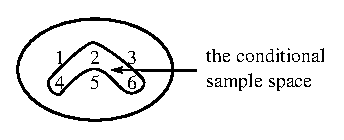
\includegraphics{figure/fig1.eps}}
\smallskip

So there are only 3 possible outcomes given an even number occurred so
$$
P(\text{6 given an even number occurred})=\dfrac{1}{3}
$$

The new sample space is called the \underline{conditional sample space}.
\end{frame}


\begin{frame}
\myheading{2. Very Important example}

Suppose you deal two cards (in the usual way without replacement). What is $P(\heart\heart)$ i.e., $P$(two hearts in a row).

Well, $P$(first heart) $=\dfrac{13}{52}$.

Now \underline{what about the second heart}?

Many of you will come up with $\sfrac{12}{51}$ and
$$
P(\heart\heart)=(\sfrac{13}{52})(\sfrac{12}{51})
$$
\end{frame}

\begin{frame}
There are \underline{TWO} theoretical points hidden in the formula.

Let's first look at
$$
P(\underbrace{\heart\text{~on~} 2^{\text{nd}}}_{\text{this isn't really correct}})=\sfrac{12}{51}
$$
What we really computed was the \underline{conditional probability}
$$
P(\heart\text{~ on~ } 2^{\text{nd}} \text{ deal } | \ \heart\text{~on first deal})=\sfrac{12}{51}
$$
\underline{Why} Given we got a heart on the first deal the conditional sample space is the ``new deck'' with 51 cards and 12 hearts so we get
$$
P(\heart\text{~ on~ } 2^{\text{nd}} \ | \ \heart\text{~ on~ } 1^{\text{st}})=\sfrac{12}{51}
$$
\end{frame}

\begin{frame}
The second theoretical point we used was the formula which we will justify formally later
\begin{align*}
P(\heart\heart) &= P(\heart\text{~ on~ } 1^{\text{st}})P(\heart\text{~ on~ }2^{\text{nd}} \ | \ \heart\text{~ on~ }1^{\text{st}})\\[3pt]
&= \binom{13}{52}\binom{12}{51}
\end{align*}

\myheading{Basic Questions}

These examples will occur repeatedly in today's lecture.
\begin{enumerate}
\item What is
$$
P(\underbrace{\heart\text{~ on~ } 1^{\text{st}} \ | \ \heart\text{~ on~ }2^{\text{nd}}}_{\text{reverse of pg. 5}})
$$
and (easier).

\item What is $P$($\heart\text{~ on~ } 2^{\text{nd}}$ with no information on what happened on the $1^{\text{st}}$).
\end{enumerate}
\end{frame}

\begin{frame}
\myheading{A Second Gold Star Problem}

If you do 1- and 2. in the way described on this page you will get a gold star and learn a lot.

\myheading{Don't use pg. 16 in Bayes Theorem}

Let $S$ = set of unordered pairs of distinct cards

Compute $\sharp (S)$.

Let $A$ = subset of pairs of hearts = $\{\heart\heart\}\subset S$.

Compute $\sharp(A)$ and $P(A)=\dfrac{\sharp(A)}{\sharp(S)}$.

Let $B$ = subset of pairs so that the second card is a heart.

Compute $\sharp(B)$ and $P(B)$ solving $2$.

Now compute $P(\heart\text{~ on~ } 1^{\text{st}} \ | \ \heart \text{~ on~ } 2^{\text{nd}})$ by taking the ratio (pg. 11) or else computing the conditional sample space.
\end{frame}

\begin{frame}
\myheading{The Formal Mathematical Theory of Conditional Probability}

\smallskip
\centering{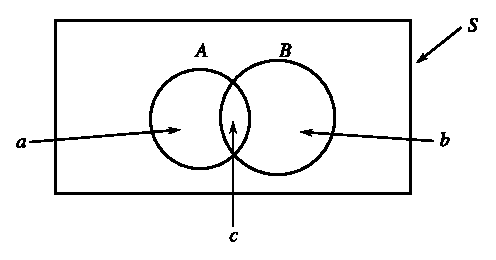
\includegraphics{figure/fig2.eps}}
\smallskip
$$
\sharp (S)=n, \ \sharp(A)=a, \ \sharp(B)=b, \ \sharp(A\cap B)=C
$$

\begin{nonumproblem}
Let $S$ be a finite set with the equally - likely probability measure and $A$ and $B$ be events with coordinalities shown in the picture.
\end{nonumproblem}
\end{frame}

\begin{frame}
\begin{nonumproblem}
Compute $P(A|B)$.

We are given $B$ occurs so the conditional sample space is $B$

\smallskip
\centering{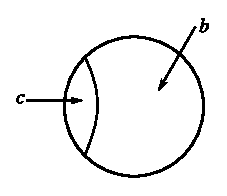
\includegraphics{figure/fig3.eps}}
\smallskip

Only part of $A$ is allowed since we know $B$ occurred namely $A\cap B$
\begin{align*}
P(A|B) &= \dfrac{\sharp(A\cap B)}{\sharp(B)}\\[3pt]
       &= \dfrac{c}{b}
\end{align*}
\end{nonumproblem}
\end{frame}

\begin{frame}
We can rewrite this as
$$
P(A|B)=\dfrac{a}{b}=\dfrac{\sfrac{a}{n}}{\sfrac{b}{n}}=\dfrac{P(A\cap B)}{P(B)}
$$
so
\begin{equation*}
P(A|B)=\dfrac{P(A\cap B)}{P(B)}\tag{*}
\end{equation*}
This intuitive formula for the equally likely probability measure leads to the following.
\end{frame}

\begin{frame}
\myheading{Formal Mathematical Definition}

Let $A$ and $B$ be any two events in a sample space $S$ with $P(B)\neq 0$. The conditional probability of $A$ given $B$ is written $P(A|B)$ and is \underline{defined} by
\begin{equation*}
P(A|B)=\dfrac{P(A\cap B)}{P(B)}\tag{*}
\end{equation*}
so if $P(A)\neq 0$ then 
\begin{equation*}
P(B|A)=\dfrac{P(B\cap A)}{P(A)}=\dfrac{P(A\cap B)}{P(A)}\tag{**}
\end{equation*}
Since $A\cap B-B\cap A$.
\end{frame}

\begin{frame}
We won't prove the next theorem but you could do it and it is useful.

\begin{nonumtheorem}
Fix $B$ with $P(B)\neq 0$. $P(\cdot | B)$ satisfies the axioms (and theorems) of a probability measure - see Lecture 1.

\myheading{For example}
\begin{enumerate}
\item $P(A_{1}\cup A_{2}|B)=P(A_{1}|B)+P(A_{2}|B)-P(A_{1}\cap A_{2}|B)$

\item $P(A'|B)=1-P(A|B)$
\end{enumerate}
$Z$\quad $P(A|\cdot)$ does not satisfy the axioms and theorems.
\end{nonumtheorem}
\end{frame}

\begin{frame}
\myheading{The Multiplicative Rule for $P(A\cap B)$}

Rewrite (**) as 
$$
P(A\cap B)=P(A)P(B|A)(\sharp)
$$
$(\sharp)$ is very important, more important then (**).

It complement the formula 
$$
P(A\cup B)=P(A)+P(B)-P(A\cap B)
$$
\underline{Now we know how $P$ interacts with the basic binary operations $\cup$ and $\cap$.}
\end{frame}

\begin{frame}
More generally
$$
P(A\cap B\cap C)=P(A)P(B|A)P(C|A\cap B)
$$

\myheading{Exercise}

Write down  $P(A\cap B\cap C\cap D)$.

\myheading{Traditional Example}

An urn contains 5 white chips, 4 black chips and 3 red chips.

Four chips are drawn sequentially without replacement. Find $P(WRWB)$.
\end{frame}

\begin{frame}
\centerline{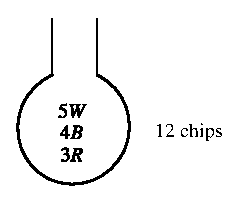
\includegraphics[scale=.9]{figure/fig4.eps}}

\begin{nonumsolution}
$P(WRWB)=\left(\dfrac{5}{12}\right)\left(\dfrac{3}{11}\right)\left(\dfrac{4}{10}\right)\left(\dfrac{4}{9}\right)$

What did we do formally 
$$
P(WRWB)=P(W)\cdot P(R|W)
$$

\underline{$P(W|W\cap R)\cdot P(B|W\cap R\cap W)$}

Now we redo the gold star problem (not the gold star way) namely we compute
$$
P(\underbrace{\heart\text{~ on~ } 1^{\text{st}}}_{A} \ | \ \underbrace{\heart\text{~ on~ }2^{\text{nd}}}_{B})
$$
\end{nonumsolution}
\end{frame}

\begin{frame}
\underline{By Definition}
$$
P(A|B)=\dfrac{P(A\cap B)}{P(B)}=\dfrac{P(\heart\heart)}{P\left(\begin{array}{c} \heart \text{~on~} 2^{\text{nd}} \text{~ with the}\\ \text{other information}\end{array}\right)}
$$
Now we know from pg. 5.
$$
P(\heart\heart)=(\sfrac{13}{52})(\sfrac{12}{51})
$$
Now we need
$$
P(\heart\text{~ on~ } 2^{\text{nd}}\text{~with no other information})=\sfrac{13}{52}
$$
We will prove this on pg. 18 - it also follows from the gold star approach on pg. 7.

So
\begin{align*}
&= P(\heart\text{~ on ~}1^{\text{st}} \ | \ \heart\text{~ on ~} 2^{\text{nd}})=\dfrac{(\cancel{\sfrac{13}{52}})(\cancel{\sfrac{12}{51}})}{(\cancel{\sfrac{13}{52}})}=\dfrac{12}{51}\\
&= P(\underbrace{\heart \text{~ on~ } 2^{\text{nd}} \ | \ \heart \text{~ on~ } 1^{\text{st}}}_{\text{pg. 5}}) !!
\end{align*}
\end{frame}

\begin{frame}
\myheading{Bayes' Theorem (pg. 72)}

Bayes' Theorem is a truly remarkable theorem. It tells you ``how to compute $P(A|B)$ if you know $P(B|A)$ and a few other things''. 

For example - we will get a new way to compute are favorite probability $P(\heart\text{~ as~ } 1^{\text{st}} \ | \ \heart \text{~ on~ } 2^{\text{nd}})$ because we know $P(\heart\text{~ on~ } 2^{\text{nd}} \ | \ \heart\text{~ on~ } 1^{\text{st}})$.

First we will need on preliminary result.
\end{frame}

\begin{frame}
\myheading{The Law of Total Probability}

Let $A_{1}$, $A_{2},\ldots,A_{k}$ be mutually exclusive

$(A_{i}\cap A_{j}=\emptyset)$ and exhaustive.

($A_{1}\cup A_{2}\cup\ldots\cup A_{k}=S=$ the whole space)

Then for any event $B$
\begin{align*}
P(B) &= P(B|A_{1})P(A_{1})+P(B|A_{2})P(A_{2})\\
     &\quad +\cdots+P(B|A_{k})P(A_{k})\tag{b}
\end{align*}
\underline{Special case} $k=2$ so we have $A$ and $A'$
\begin{equation*}
P(B)=P(B|A)P(A)+P(B|A')P(A')\tag{bb}
\end{equation*}
\end{frame}

\begin{frame}
Now we can \underline{prove}

$P$($\heart$ on $2^{\text{nd}}$ with no other information) = $\sfrac{13}{52}$
\begin{align*}
\text{Put}\quad B &= \heart\text{~ on~ } 2^{\text{nd}}\\[3pt]
                A &= \text{heart on~ } 1^{\text{st}}\\[3pt]
                A' &= \text{a nonheart on } 1^{\text{st}}
\end{align*}
Lets write $\cancel{\heart}$ for nonheart.

So,
\begin{gather*}
P(\cancel{\heart}\text{~ on~ } 1^{\text{st}})=\sfrac{39}{52}\\[3pt]
P(\heart\text{~ on~ } 2^{\text{nd}}/\cancel{\heart}\text{~ on first})=\sfrac{13}{51}
\end{gather*}
\end{frame}

\begin{frame}
Now
\begin{align*}
P(B) &= P(B|A)P(A)+P(B|A')P(A')\\[3pt]
     &= P(\heart\text{~ on ~} 2^{\text{nd}} \ | \ \heart \text{~ on~ } 1^{\text{st}})P(\heart \text{~ on~ } 1^{\text{st}})\\[3pt]
&\quad +P(\heart\text{~ on~ }2^{\text{nd}} \ | \ \cancel{\heart}\text{~ on~ } 1^{\text{st}})P(\cancel{\heart}\text{~ on~ } 1^{\text{st}})\\[3pt]
&= (\sfrac{12}{51})(\sfrac{13}{52})+(\sfrac{13}{51})(\sfrac{39}{52})\\
\intertext{add fractions}\\
&= \dfrac{(12)(13)+(13)(39)}{(51)(52)}\\
\intertext{factor out 13 add to get 51}\\
&= \dfrac{(13)\displaystyle{\mathop{(12+39)}\limits^{\myarrow}}}{(51)(52)}=\dfrac{(13)(\cancel{51})}{\cancel{(51)}(52)}\\[5pt]
&= \sfrac{(13)}{(52)}\qquad \text{Done!}
\end{align*}
\end{frame}

\begin{frame}
(b) is ``very easy'' to prove but we won't do it.

Now we can state Bayes' Theorem.

\myheading{Bayes' Theorem (pg. 73)}

Let $A_{1},A_{2},\ldots,A_{k}$ be a collection of $n$ mutually exclusive and exhaustive events with $P(A_{i})>0$

$i=1,2,\ldots,k$. Then for any event $B$ with $P(B)>0$
$$
P(A_{j}|B)=\dfrac{P(B|A_{j})P(A_{j})}{\sum\limits^{k}_{i=1}P(B|A_{i})P(A_{i})}
$$
Again we won't give the proof.
\end{frame}

\begin{frame}
\myheading{Special Case $k=2$}

Suppose we have two events $A$ and $B$ with $P(A)>0$, $P(A')>0$ and $P(B>0)$. Then
$$
\sharp)P(A|B)=\dfrac{P(B|A)P(A)}{P(B|A)P(A)+P(B|A')P(A')}
$$
Now we will compute (for the last time)
$$
P(\heart\text{~ on~ } 1^{\text{st}} \ | \ \heart\text{~ on~ } 2^{\text{nd}})
$$
Using Bayes' Theorem.

This is the obvious way to
\end{frame}

\begin{frame}
do it since we know the probability ``the other way around''
$$
P(\heart\text{~ on~ } 2^{\text{nd}} \ | \ \heart \text{~ on ~} 1^{\text{st}})=\sfrac{12}{51}
$$
So let's do it.
\begin{align*}
\text{We put~ } A &= \heart \text{~ on~ } 1^{\text{st}}\\
\text{so~ }    A' &= \cancel{\heart}\text{~ on~ } 1^{\text{st}}\\
\text{and~ } B &= \heart\text{~ on second}
\end{align*}
plugging into $(\sharp)$ we get 
\begin{align*}
& P(\heart\text{~ on~ } 1^{\text{st}} \ | \ \heart\text{~ on~ } 2^{\text{nd}})\\
& = \dfrac{P(\heart\text{~ on~ } 2^{\text{nd}} \ | \ \heart\text{~ on ~} 1^{\text{st}})P(\heart\text{~ on~ } 1^{\text{st}})}{P(\heart\text{~ on~ } 2^{\text{nd}} \ | \ \heart\text{~ on~ } 1^{\text{st}})P(\heart\text{~ on~ } 1^{\text{st}})+P(\heart\text{~ on~ } 2^{\text{nd}} \ | \ \cancel{\heart}\text{~ on~ } 1^{\text{st}})P(\cancel{\heart}\text{~ on~ } 1^{\text{st}})}
\end{align*}
\end{frame}

\begin{frame}
\centerline{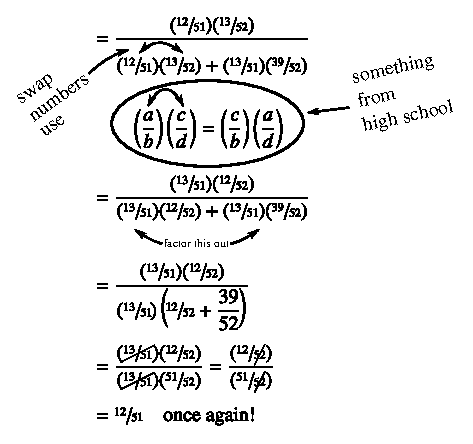
\includegraphics{figure/fig5.eps}}
%\begin{align*}
%&= \dfrac{(\sfrac{12}{51})(\sfrac{13}{52})}{(\sfrac{12}{51})(\sfrac{13}{52})+(\sfrac{13}{51})(\sfrac{39}{52})}\\[10pt]
%&\qquad \left(\dfrac{a}{b}\right)\left(\dfrac{c}{d}\right)=\left(\dfrac{c}{b}\right)\left(\dfrac{a}{d}\right)\\[10pt]
%&=\dfrac{(\sfrac{13}{51})(\sfrac{12}{52})}{(\sfrac{13}{51})(\sfrac{12}{52})+(\sfrac{13}{51})(\sfrac{39}{52})}\\[10pt]
%&= \dfrac{(\sfrac{13}{51})(\sfrac{12}{52})}{(\sfrac{13}{51})(\sfrac{12}{52}+\dfrac{39}{52})}\\[10pt]
%&= \dfrac{(\cancel{\sfrac{13}{51}})(\sfrac{12}{52})}{(\cancel{\sfrac{13}{51}})(\sfrac{51}{52})}=\dfrac{(\sfrac{12}{\cancel{52}})}{(\sfrac{51}{\cancel{52}})}\\[10pt]
%&= \sfrac{12}{51}\quad \text{once again!}
%\end{align*}
\end{frame}

\begin{frame}
The algebra was hard but the approach was the most natural - a special case of 

\smallskip
\underline{General Principle}
\smallskip

If you know $P(B|A)$ and you want to compute $P(A|B)$ use Bayes' Theorem in the $(\sharp)$ version, pg. 22.

\myheading{Compulsory Reading (for your own heath)}

In case you or someone you love tests positive for a \underline{rare} (this is the point) disease, read Example 2.30, pg. 73. Misleading (and even bad) statistics is rampant in medicine.
\end{frame}
\end{document}


